\section{Exercise 1}

\subsection{Requirements}
\label{subsec:requirements}

The \href{https://github.com/IsacPasianotto/cloud-computing-assignment/blob/main/exercise01/assignment.md}{assignment} requires the deployment of a scalable and secure file storage system. In particular the requirements are:

\begin{enumerate}
    \itemsep0em
    \item \textit{Management of user authentication and authorization}
    \begin{enumerate}
        \itemsep0em
        \item User should be able to sing up, log in and log out [\ref{subsec:nextcloud}]
        \item User should have different roles, i.e. admin and regular user [\ref{subsec:nextcloud}]
        \item Admin should be able to create, delete and modify users [\ref{subsec:nextcloud}]
        \item Regular user should have access to a personal storage space [\ref{subsec:nextcloud}]
    \end{enumerate}

    \item \textit{Management of file operations}
    \begin{itemize}
        \itemsep0em
        \item User should be able to upload, download, delete and modify from their private storage space [\ref{subsec:nextcloud}]
    \end{itemize}

    \item \textit{Scalability}
    \begin{enumerate}
        \itemsep0em
        \item The designed system should handle a growing number of users and files [\ref{subsec:deployment-real-world}]
        \item A theoretical discussion about the way to increase load and traffic [\ref{subsubsec:approach-independent}]
    \end{enumerate}

    \item{Security}
    \begin{enumerate}
        \itemsep0em
        \item The secure file storage and transmission should be implemented [\ref{subsec:security}]
        \item Discussion about how to secure user authentication [\ref{subsec:security}, \ref{subsec:deployment}]
        \item Discussion about measures to prevent unauthorized access [\ref{subsec:security}]
    \end{enumerate}

    \item{Cost-effectiveness}
    \begin{itemize}
        \itemsep0em
        \item Discussion about the costs implications of the designed system and how to optimize them [\ref{subsubsec:iaas}, \ref{subsubsec:paas}, \ref{subsubsec:saas}, \ref{subsubsec:cloudless}]
    \end{itemize}

    \item{Deployment}
    \begin{enumerate}
        \itemsep0em
        \item Provision of containerized environment based on docker [\ref{subsec:deployment}]
        \item Choice of a cloud provider to deploy the system in a production scenario [\ref{subsec:deployment-real-world}]
    \end{enumerate}

    \item{Testing}
    \begin{enumerate}
        \itemsep0em
        \item Assessment of the system performance: load [\ref{subsubsec:test}]
        \item Assessment of the system performance: I/O  [\ref{subsubsec:test}]
    \end{enumerate}
\end{enumerate}

Following the assignment suggestion, the presented solution will be based on the \href{https://nextcloud.com/}{Nextcloud} platform.

\subsection{Technical deployment details}
\label{subsec:deployment}

The deployment of the system is based on the use of \href{https://www.docker.com/}{Docker} containers.
In particular, since more than one container is used, the \href{https://docs.docker.com/compose/}{\texttt{docker-compose}} tool is used to manage the deployment.
The complete of the multi-container setting configuration is done in the \href{https://github.com/IsacPasianotto/cloud-computing-assignment/blob/main/exercise01/docker-compose.yaml}{\texttt{docker-compose.yaml}} file.
All the user container are taken from the \href{https://hub.docker.com/}{Docker Hub} and properly configured, no custom images are used.

All the container shares the same network called \texttt{nextcloud\_network}, which can be created with:

\begin{lstlisting}[language=bash]
$ docker network create nextcloud_network
\end{lstlisting}

\subsubsection{Used images}
The \texttt{docker-compose.yml} file uses the following images\footnote{This configuration is heavily inspired by one of the \href{https://github.com/nextcloud/docker/blob/master/.examples/docker-compose/with-nginx-proxy/mariadb/fpm/docker-compose.yml}{examples provided by the Nextcloud team}.}:

\begin{enumerate}
    \itemsep0em
    \item \href{https://hub.docker.com/layers/library/nextcloud/28.0.2-fpm/images/sha256-dc1b232c39cd29fe81442f0e4d1c523148afecaf0bcf1cdffb7c52441bf63af7?context=explore}{\texttt{nextcloud:28.0.2-fpm}}: 
    base image for the Nextcloud platform. In particular two images are used, the principal one for having the desired storage platform and a second one which is going to run the built-in \texttt{cron.sh}  script for background tasks\footnote{This solution was inspired by \href{https://help.nextcloud.com/t/nextcloud-docker-container-best-way-to-run-cron-job/157734/2}{this} and \href{https://help.nextcloud.com/t/clarification-regarding-cron-jobs-setup-config/134450}{this} forum pages}.
    \item \href{https://hub.docker.com/_/mariadb}{\texttt{mariadb:11.2.3}}: the databases the official Nextcloud documentation suggests to use. 
    \item \href{https://hub.docker.com/_/nginx}{\texttt{nginx:1.25.4-alpine3.18}}: the web server used to serve the Nextcloud platform, the other alternative were apache.
    \item \href{https://hub.docker.com/_/redis}{\texttt{redis:7.2.4-alpine}}: the cache server; when a client requests a file, the server will first check if the file is in the cache, this should enhance the performance.
    \item \href{https://hub.docker.com/_/caddy}{\texttt{caddy:2.7.6-alpine}}: a lightweight web server, used as a reverse proxy. It was chosen because it automatically manages the SSL certificate[\ref{subsec:security}].
\end{enumerate}

Three volumes are used to store the data: \texttt{nextcloud\_data}, \texttt{db\_data} and \texttt{caddy\_data}. 
To run the project, first create those volumes with: \texttt{docker volume <volume\_name>}, then run\footnote{If your system relies on \href{https://www.redhat.com/en/topics/linux/what-is-selinux}{SELinux}, this will probably cause some issues. For the purpose of this exercise, I've just disabled it with \texttt{sudo setenforce 0}. In a production environment, it should be properly configured.}:
\begin{lstlisting}[language=bash]
$ docker-compose up -d
\end{lstlisting}
The \texttt{docker-compose} tool will create the containers, then the system will be ready to use and accessible at \texttt{https://localhost}\footnote{A self-signed certificate is used, so the browser will show a warning.}; the first time the system is accessed, the user will be asked to create an admin account.

\subsection{Nextcloud characteristics}
\label{subsec:nextcloud}

Nextcloud offers out-of-the-box all the functionalities required at \hyperref[subsec:requirements]{points 1 and 2} of the requirements.

Using the provided web interface, the admin can create, delete and modify users.
Obviously, every created user can log in, log out to the system.
Every user (normal or admin) has access to a personal storage space, where they can upload, download, delete and modify files that are not accessible by other users.

The admin can also limited the storage space available to each user (default no limitation, but 1GB, 5GB, 15GB quotas are available).

\subsection{Security measures}
\label{subsec:security}

\subsubsection{Storage security}
Nextcloud software comes with a lot of security features which can help to fulfill the requirements at \hyperref[subsec:requirements]{point 4}.
First of all, for what regards the secure file storage, there is the possibility to enable the server-side encryption, which encrypts the files before they are uploaded to the server.
This can be activated both form the web interface with a admin account (\textit{Administration settings} $\rightarrow$ \textit{Administration Security} $\rightarrow$ \textit{Server-side encryption})
or from the command line with the \href{https://docs.nextcloud.com/server/latest/admin_manual/configuration_server/occ_command.html}{\texttt{occ}} command:

\begin{lstlisting}[language=bash, basicstyle=\footnotesize]
$ docker exec --user www-data nextcloud-app /var/www/html/occ app:enable encryption
$ docker exec --user www-data nextcloud-app /var/www/html/occ encryption:enable
$ # to encrypt all the files already uploaded: 
$ echo "yes" | docker exec -i --user www-data nextcloud-app /var/www/html/occ encryption:encrypt-all
\end{lstlisting}

\subsubsection{User authentication security}
Moreover, Nextcloud provides useful features to enhance the security of the user authentication; in the same \textit{Administration Security} section mentioned above, the admin can enable: 

\begin{itemize}
    \itemsep0em
    \item Enforce the use of both upper and lower case letters, enforce the use of numbers and enforce the use of special characters in the user password;
    \item Forbid the use of common passwords;
    \item Set the minimum length of the password;
    \item Check the password against the \href{https://haveibeenpwned.com/}{haveibeenpwned.com} database.
    \item Tune the number of days after which the user is forced to change the password and the history of the password (i.e. the user cannot use the same password for a certain number of times).
    \item Enable the two-factor authentication.
\end{itemize}

Additionally, Nextcloud is compatible with  \href{https://oauth.net/2/}{OAuth 2.0} protocol, which can be used to authenticate the user with a third-party service, and it has an actionable app to prevent brute force attacks.

\subsubsection{SSL certificate}

All the already mentioned security measures can only guarantee a good security from the server side. In a real-world scenario, the server will not be the \texttt{localhost}, but most likely a domain name.
In this case, a critical point is the communication between the user's browser (or client) and the server itself. 
This is the reason why in the \texttt{docker-compose.yaml} file, the \texttt{caddy} container is used. In fact it automatically manages the SSL certificate, so the communication between the user and the server is encrypted and uses the HTTPS protocol.

\subsection{Test of the infrastructure}
\label{subsec:test}
\subsubsection{Load test}
\label{subsubsec:test}

To perform a load test, I've used the \href{https://locust.io/}{\texttt{locust}} testing tool. It is a Python library that allows to define a set of user behaviors and then simulate a large number of users that perform those behaviors.

In the \href{https://github.com/IsacPasianotto/cloud-computing-assignment/blob/main/exercise01/locust/realistic-scenario.py}{\texttt{realistic-scenario.py}} I have defined a set of behaviors that a user can perform which are: 


\begin{center}
    \begin{tabular}{lrl}
        \hline
        Task & Probability & Description \\
        \hline
        \texttt{upload\_small} & 30\% & Upload a small file: 13.5KB \\
        \texttt{upload\_medium} & 35\% & Upload a medium file: 42.0MB \\
        \texttt{upload\_large} & 5\% & Upload a large file: 1.0GB \\
        \texttt{download} & 30\% & Download the medium file \\
        \hline
    \end{tabular}
\end{center}

I've performed the test on my laptop, which as a \href{https://www.intel.com/content/www/us/en/products/sku/193555/intel-core-i58365u-processor-6m-cache-up-to-4-10-ghz/specifications.html}{Intel Core i5-8365U} CPU and 2$\times$8GB of DDR4 RAM.
Locust was set to spawn a user each second, up to a given upper limit, and at each second, for all the currently spawned users, try to perform one of the above tasks.

It toured out that my hardware was able to handle up to 20 users without any issue, but when the number of users was increased to 30, the system started to show the "\textit{429: Too Many Requests}" error\footnote{It's also worth to be mentioned that warning about usage over 90\% of the CPU.}, see \hyperref[fig:locust-load-tests]{Figure \ref{fig:locust-load-tests}}. 

\begin{figure}[H]
    \centering
    \begin{subfigure}{0.49\textwidth}
        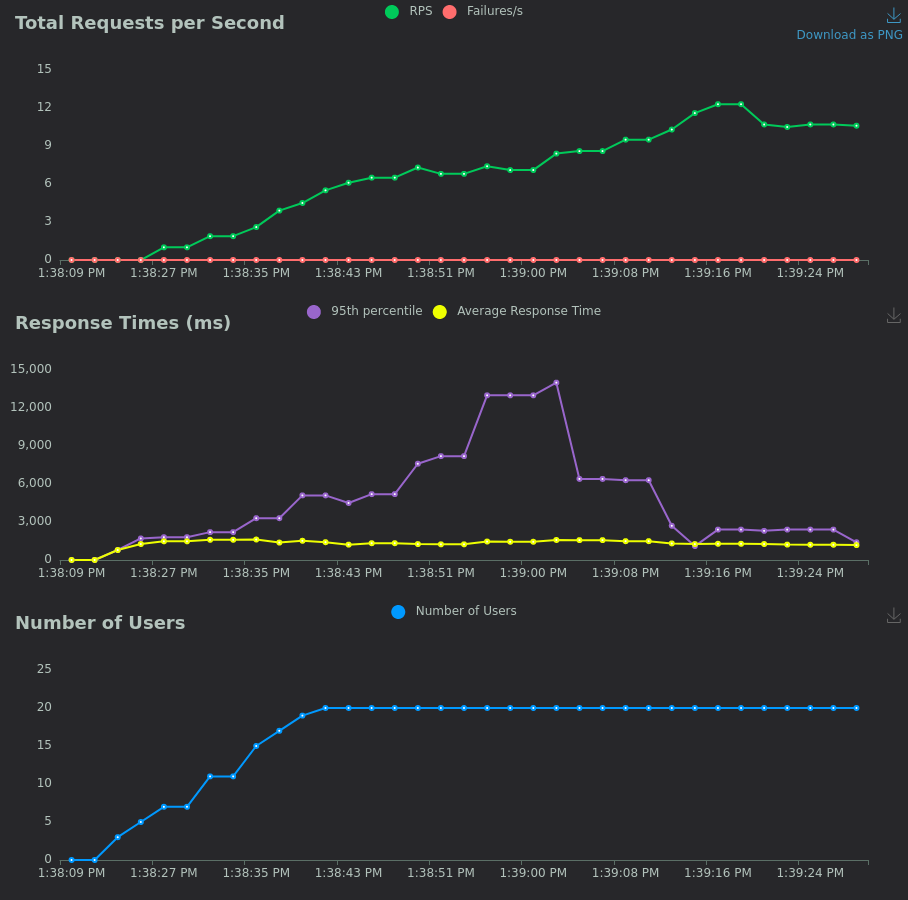
\includegraphics[width=\linewidth]{./images/ex1/20-users.png}
        \caption{Load test with 20 users, no failures are reported}
        \label{fig:locust-20-users}
    \end{subfigure}
    \hfill
    \begin{subfigure}{0.49\textwidth}
        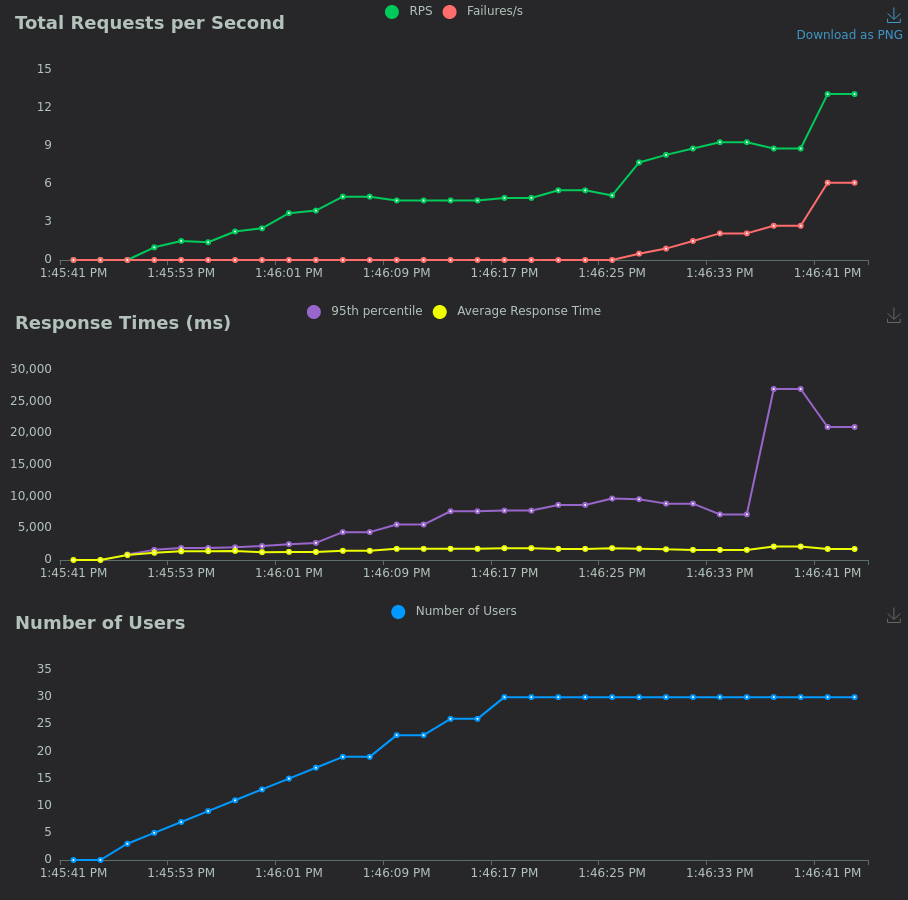
\includegraphics[width=\linewidth]{./images/ex1/30-users.png}
        \caption{Load test with 30 users, failures start to appear as all the users are spawned}
        \label{fig:locust-30-users}
    \end{subfigure}
    \caption{Comparison of load tests with different user counts}
    \label{fig:locust-load-tests}
\end{figure}

\subsubsection{I/O test}
\label{subsubsec:test}

To asses the I/O traffic, I've used the \href{https://docs.docker.com/config/containers/runmetrics/}{\texttt{docker stats}} tool, which provides a real-time view of the CPU, memory, network, and disk I/O usage of the running containers.
During the load test reported in the \hyperref[fig:locust-load-tests]{Figure \ref{fig:locust-load-tests}}, the I/O traffic was monitored in this way. The result is shown in \hyperref[fig:docker-stats]{Figure \ref{fig:docker-stats}}.

\begin{figure}[H]
    \centering
    \begin{subfigure}{\textwidth}
        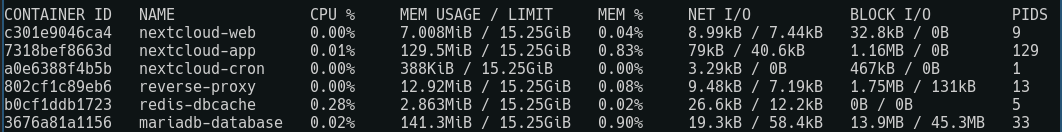
\includegraphics[width=\linewidth]{./images/ex1/newspawedIO}
        \caption{Situation at newly spawned containers}
        \label{fig:newspawedIO}
    \end{subfigure}
    \begin{subfigure}{\textwidth}
        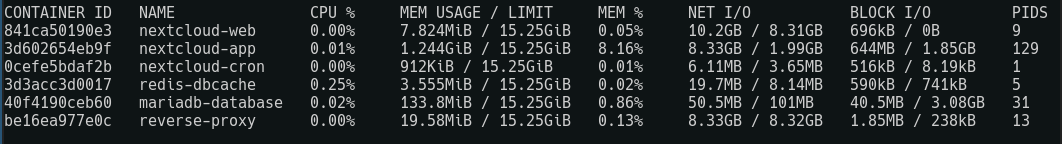
\includegraphics[width=\linewidth]{./images/ex1/20usersIO}
        \caption{20 users performing 1 action per second, 60 seconds}
        \label{fig:20usersIO}
    \end{subfigure}
    \begin{subfigure}{\textwidth}
        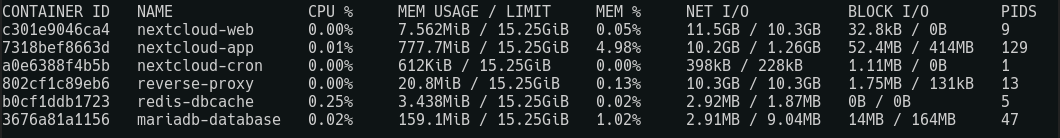
\includegraphics[width=\linewidth]{./images/ex1/30usersIO}
        \caption{30 users performing 1 action per second, 60 seconds}
        \label{fig:30usersIO}
    \end{subfigure}
    \caption{I/O traffic during the load test}
    \label{fig:docker-stats}
\end{figure}

We can see that the container which are most stressed are the proxy the web server and the nextcloud app, which is the one that handles requests
The database server is not stressed. This can be explained by the fact that the database is used to store the metadata of the files, and not the files themselves, so the I/O traffic is lower. 

\subsection{Deployment plans for hypothetical real-world scenario}
\label{subsec:deployment-real-world}

In a real-world scenario, the requirements of the system will be much higher than the one of the test, but also the resources available will be much higher.
In order to scale this solution to a production scenario some paths can be followed. 

\subsubsection{Approach-independent considerations}
\label{subsubsec:approach-independent}

Imaging a much higher traffic, some primary considerations can be made: 
first of all, some of the containers can be scaled vertically (i.e. increase the resources available to the container), for example the \texttt{redis} container, which is used as a cache server, in this way the cache hit rate will be increased, and the communication with the database will be reduced.
Also the \texttt{caddy} container can be scaled vertically, in order to handle more SSL connections.

Since \texttt{caddy} acts also as a reverse proxy, it can be used to balance the traffic among the different instances of the \texttt{nextcloud} and \texttt{nginx} containers which means that more than one instance of the \texttt{nextcloud} and \texttt{nginx} containers can be used, allowing to scale horizontally the system and distributing the traffic among the different instances.
Finally, also the database can be scaled horizontally, in order to handle more requests and to guarantee more reliability.

In addition to that, an evaluation about the trade-off between security and performance should be made. The server-side encryption can be disabled, in order to reduce the CPU usage, but this will reduce the security of the system. The possibility of disabling it and leave to the users the responsibility of encrypting the files which must be kept secret should be evaluated.

\subsubsection{On-site approach}
\label{subsubsec:cloudless}
Assuming that the organization has its own data center, the system can be deployed on it. 

\textit{Advantages}:
\begin{itemize}
    \itemsep0em
    \item The organization has full control over the infrastructure;
    \item The costs are fully predictable, easier to manage and optimize; 
    \item The data are stored in the organization's data center, so the organization has full control over them.
    \item The organization does not have to rely on a third-party organization and adopt its own policies, procedures and security measures.
\end{itemize}
\textit{Disadvantages}:
\begin{itemize}
    \itemsep0em
    \item The organization has to manage the infrastructure, which can be complex and expensive;
    \item The organization has to manage the security of the infrastructure, which can be complex and expensive;
    \item The organization must take care of the scalability of the project all by itself.
    \item The initial investment to purchase the hardware can be high.
\end{itemize}

\subsubsection{IaaS approach}
\label{subsubsec:iaas}
Assuming that the organization does not have its own data center, and considering the cost of acquiring and maintaining it too high, the system can be deployed on a cloud provider. 

In the case of \textit{Infrastructure as a Service} (IaaS) approach, the organization can rent the resources needed with the "pay as you go" model. 
Still on the organization to manage the rented resources, install and configure the system to run the wanted software.

\textit{Advantages}:
\begin{itemize}
    \itemsep0em
    \item The organization does not have to invest in hardware;
    \item The scale-up and scale-down of the resources is easy and fast;
    \item The organization does not have to manage the physical infrastructure, which can be complex and expensive;
    \item The provider can offer a object storage service, that is a reliable and scalable way to store the files which offers also backup and disaster recovery features.
\end{itemize}
\textit{Disadvantages}:
\begin{itemize}
    \itemsep0em
    \item The price of the resources could be less predictable; 
    \item The renter may increase the price of the resources;
    \item The organization still to take care of the security of the system it is running;
    \item There are risks leaved to the provider the organization has to rely on (eg. Network, "zero-day" vulnerabilities for the hypervisor, etc.);
    \item The data are not physically stored in the organization's data center;
\end{itemize}

\subsubsection{PaaS approach}
\label{subsubsec:paas}
In this case (\textit{Platform as a Service}), the organization can rent a platform where the vendor takes care of the hardware infrastructure, but also to installing and configuring the software.
In this scenario, theoretically, the organization just needs to manage the application and the data, and the vendor will take care of the rest.

\textit{Advantages}:
\begin{itemize}
    \itemsep0em
    \item The organization does not have to invest in hardware and in time to configure it to properly run the software;
    \item The organization need to manage only the application and the data;
    \item Most of the security measures which are needed are on the vendor side;
    \item The organization can rely on the vendor to take care of the scalability of the system.
\end{itemize}
\textit{Disadvantages}:
\begin{itemize}
    \itemsep0em
    \item The more the vendor takes care of, the more you pay: this solution should be the more expensive w.r.t. the IaaS and on-site approaches;
    \item The more the vendor takes care of, the less control the organization has over the infrastructure, and the more it has to trust the vendor for the security concerns;
    \item The data are not physically stored in the organization's data center;
\end{itemize}

\subsubsection{SaaS approach}
\label{subsubsec:saas}
Finally, the organization can rent a software as a service. In this case the organization does not have to manage anything, just to use the software with the features provided by the vendor and pay for it.

\textit{Advantages}:
\begin{itemize}
    \itemsep0em
    \item The organization does not have to invest in hardware and in time to configure it to properly run the software;
    \item The organization does not have to manage the application and the data, which can be time-consuming and expensive;
    \item The organization does not have to manage the security of the system;
    \item The organization does not have to manage the scalability of the system;
\end{itemize}
\textit{Disadvantages}:
\begin{itemize}
    \item Probably the most expensive solution;
    \item The organization has no control (and probably no knowledge) about the infrastructure and the security measures;
    \item The organization must completely rely on the vendor for the security and the reliability of the system;
\end{itemize}




% \subsection{Conclusions}
% \label{subsec:conclusions}
